% ! TeX program = lualatex

\documentclass{homework}
% \usepackage{lua-visual-debug}
\usepackage{graphicx}

\usepackage{macros-common}

\title{Quiz 2}
\subject{MAS109(E,F) Introduction to Linear Algebra}
\studentid{20170058}
\name{Keonwoo Kim}
\date{\today}

\begin{document}
\maketitle
\setlength{\parindent}{0pt}
\vspace*{-0.8cm}
{\Large\bf Problems}

\begin{center}
    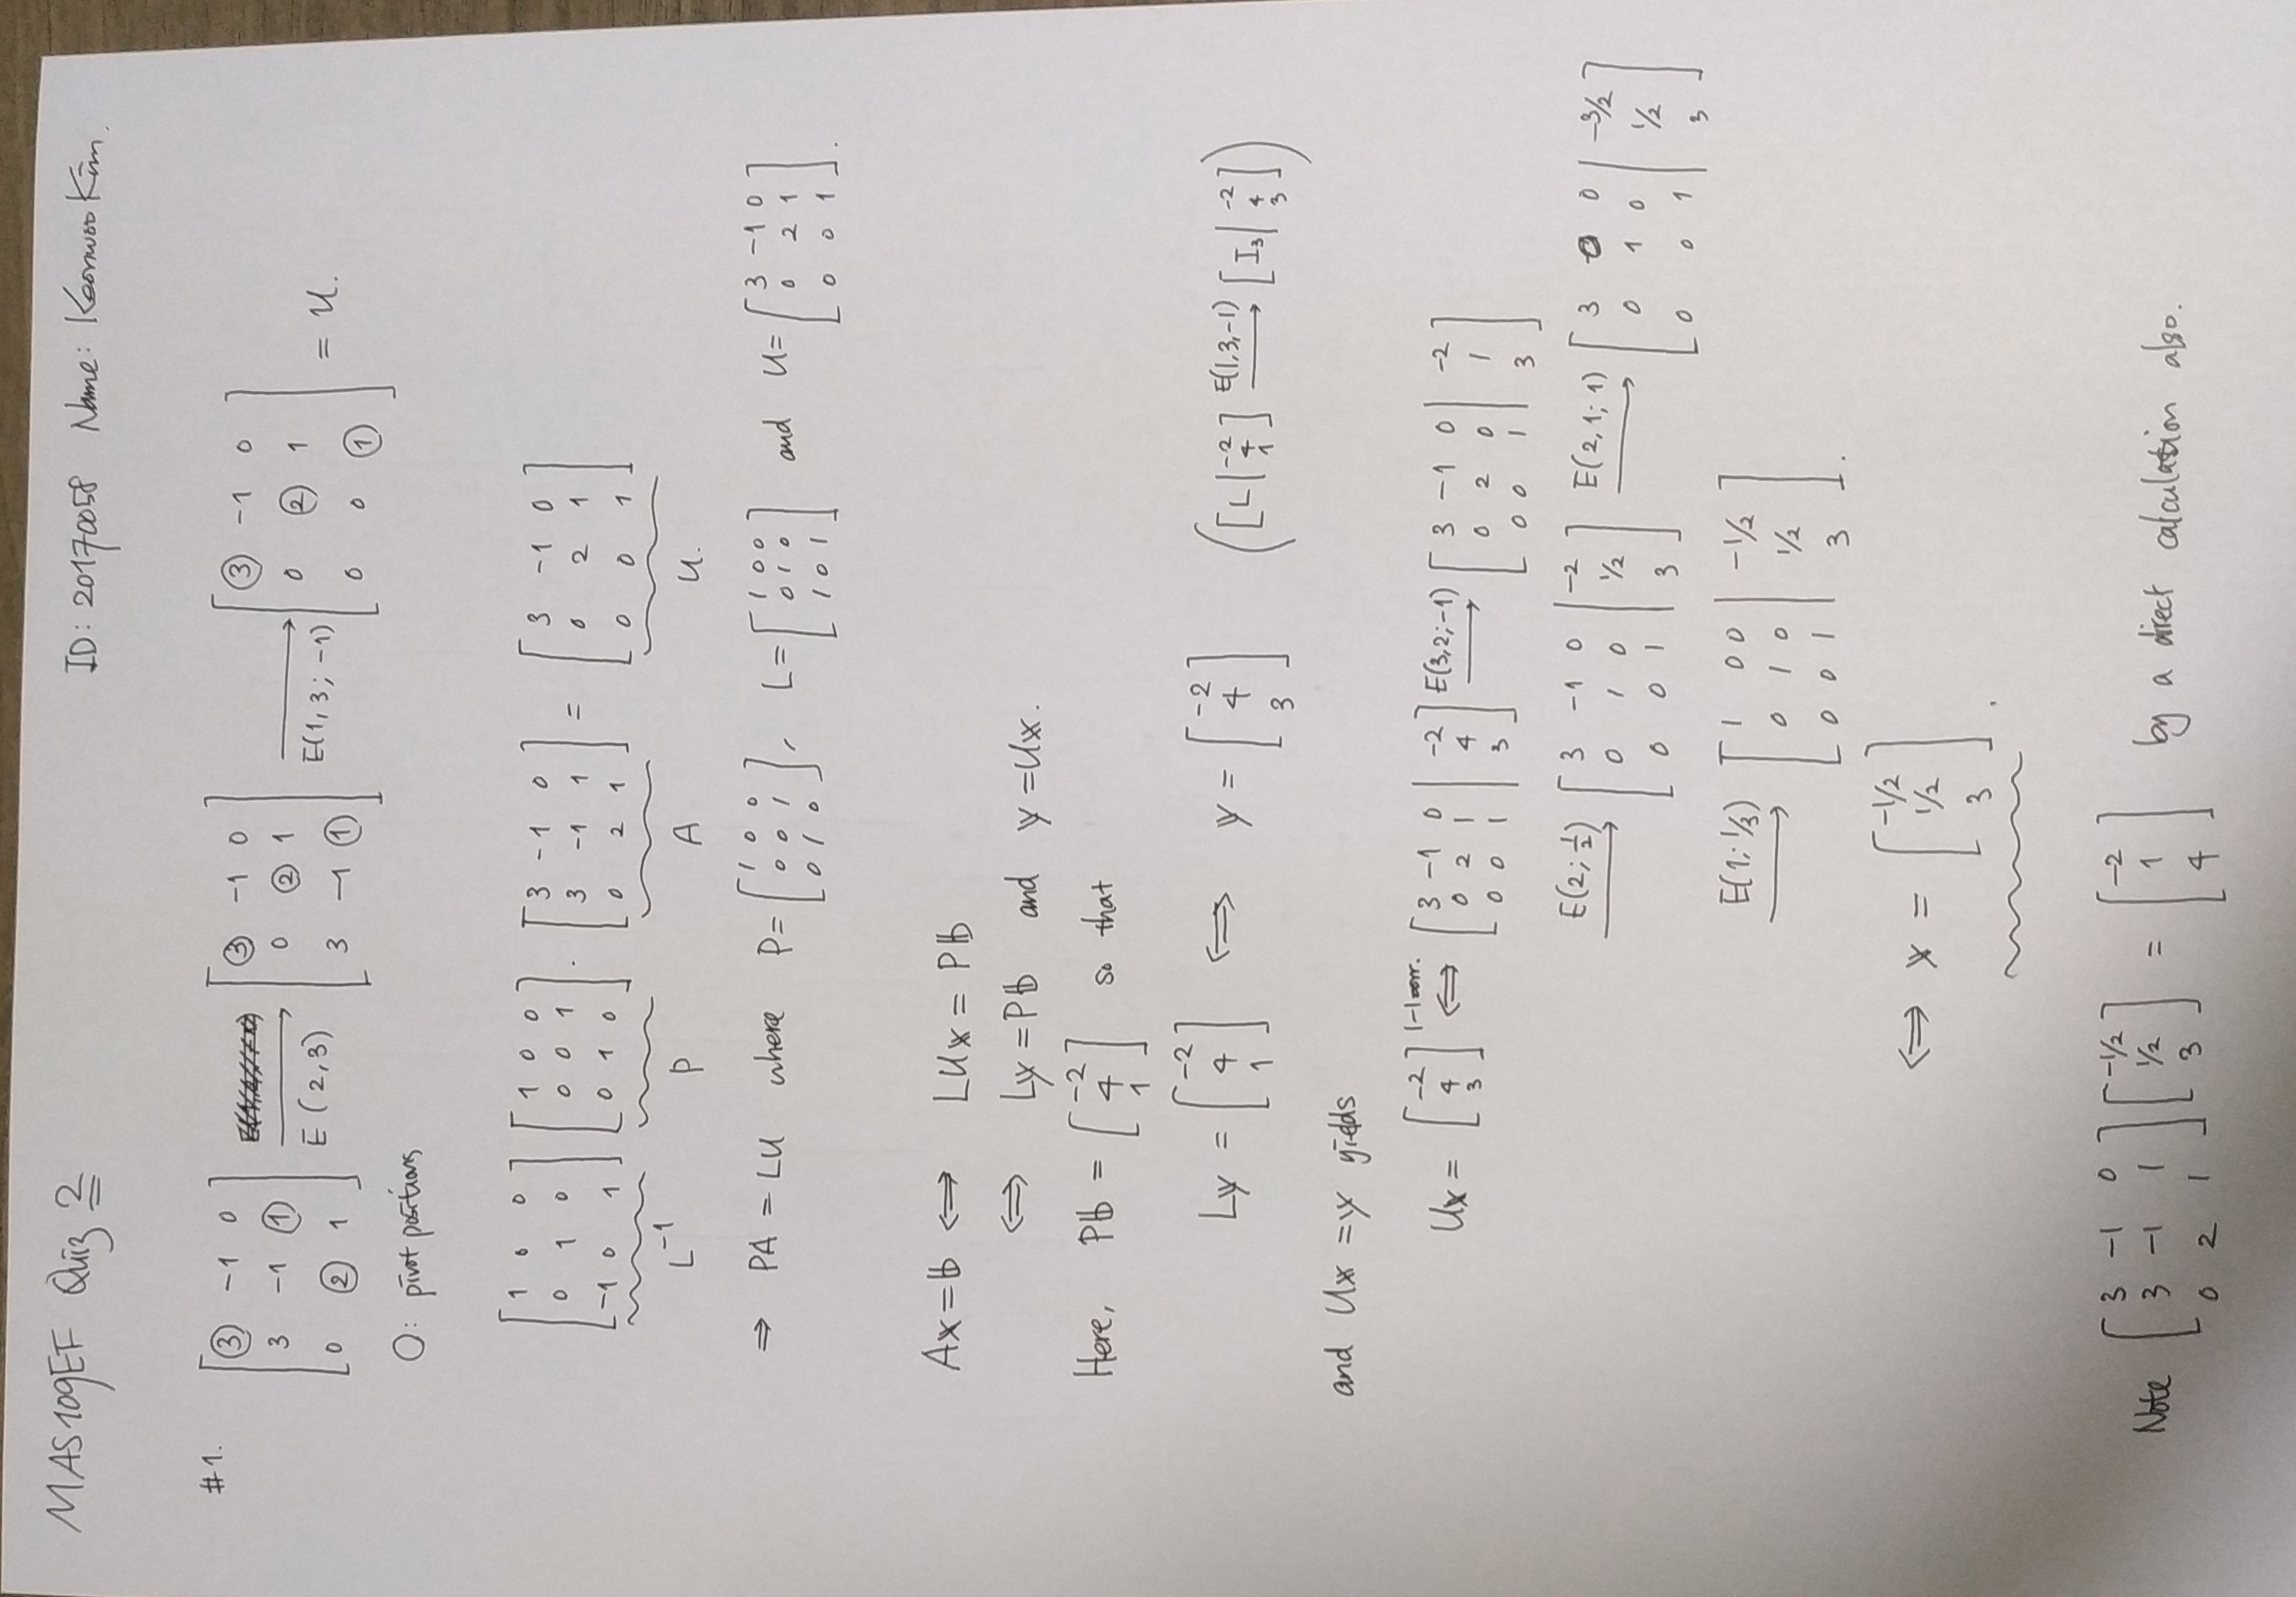
\includegraphics[height=0.9\textwidth,angle=-90,origin=c]{prob1.jpg}
\end{center}
\newpage
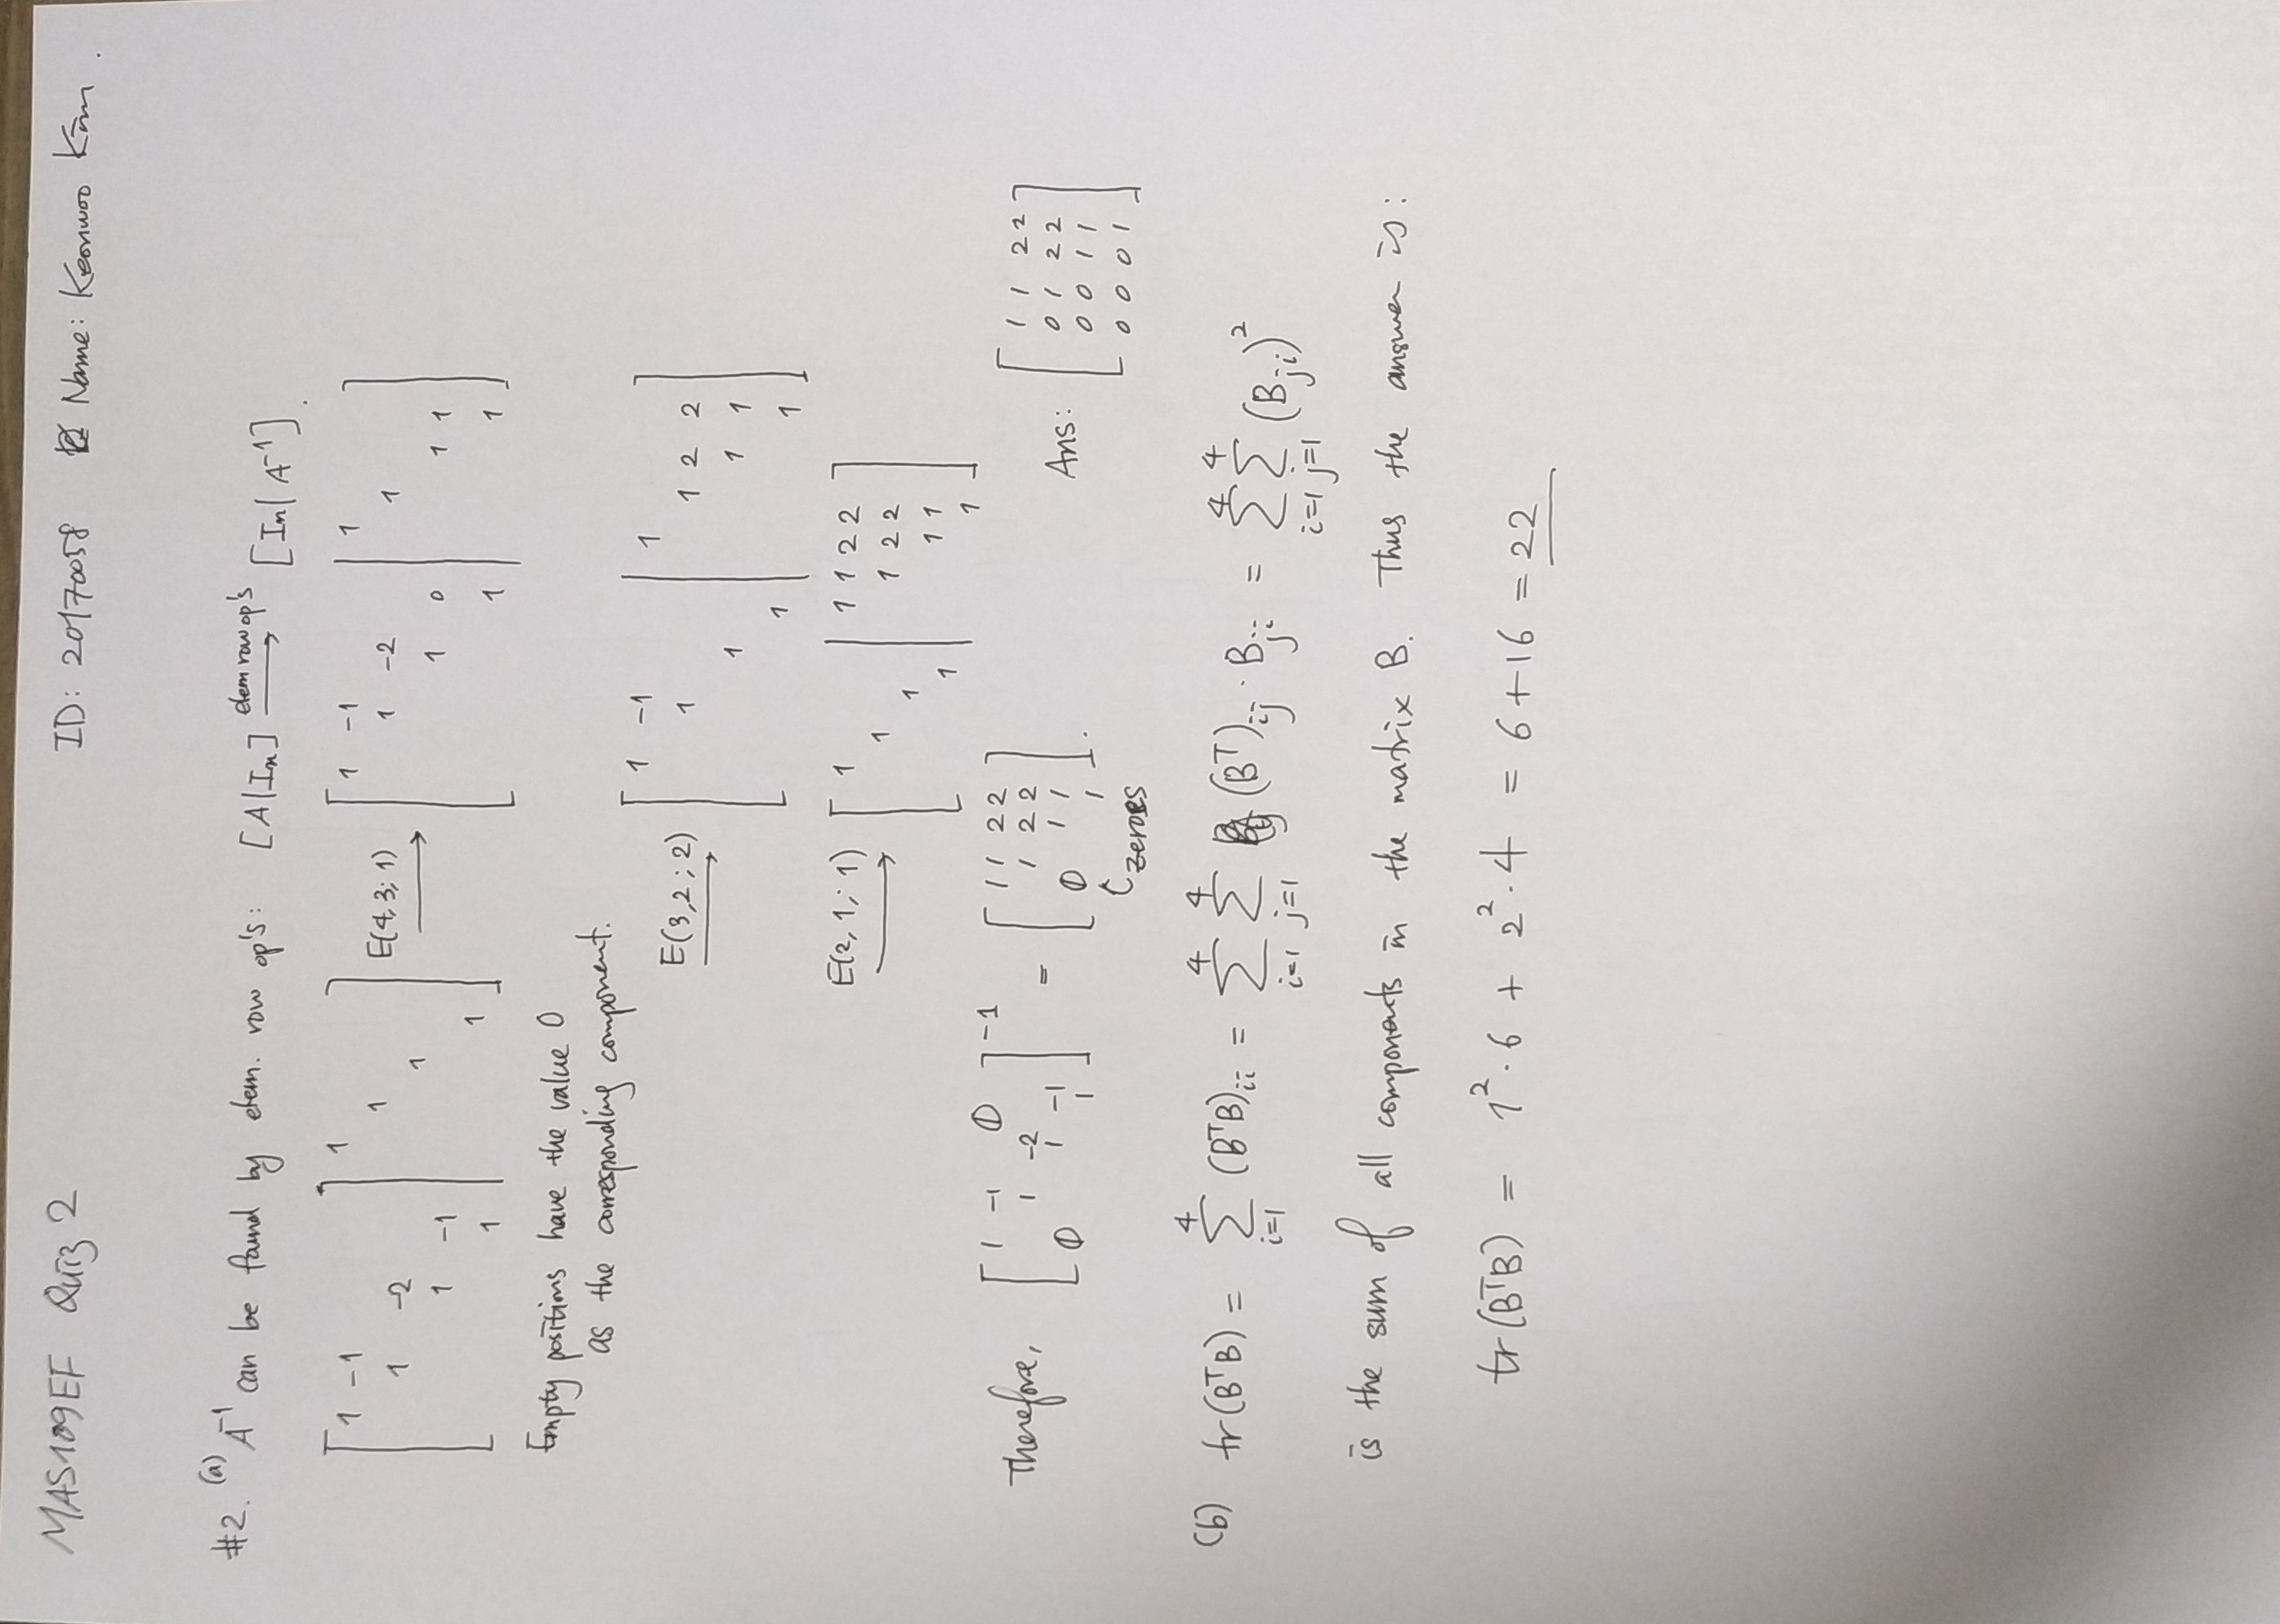
\includegraphics[height=\textwidth,angle=-90,origin=c]{prob2.jpg}
\vskip1em
*the sum of all components $\to$ the square sum of all components
\newpage

\vspace*{-0.5cm}
{\Large\bf Summary}

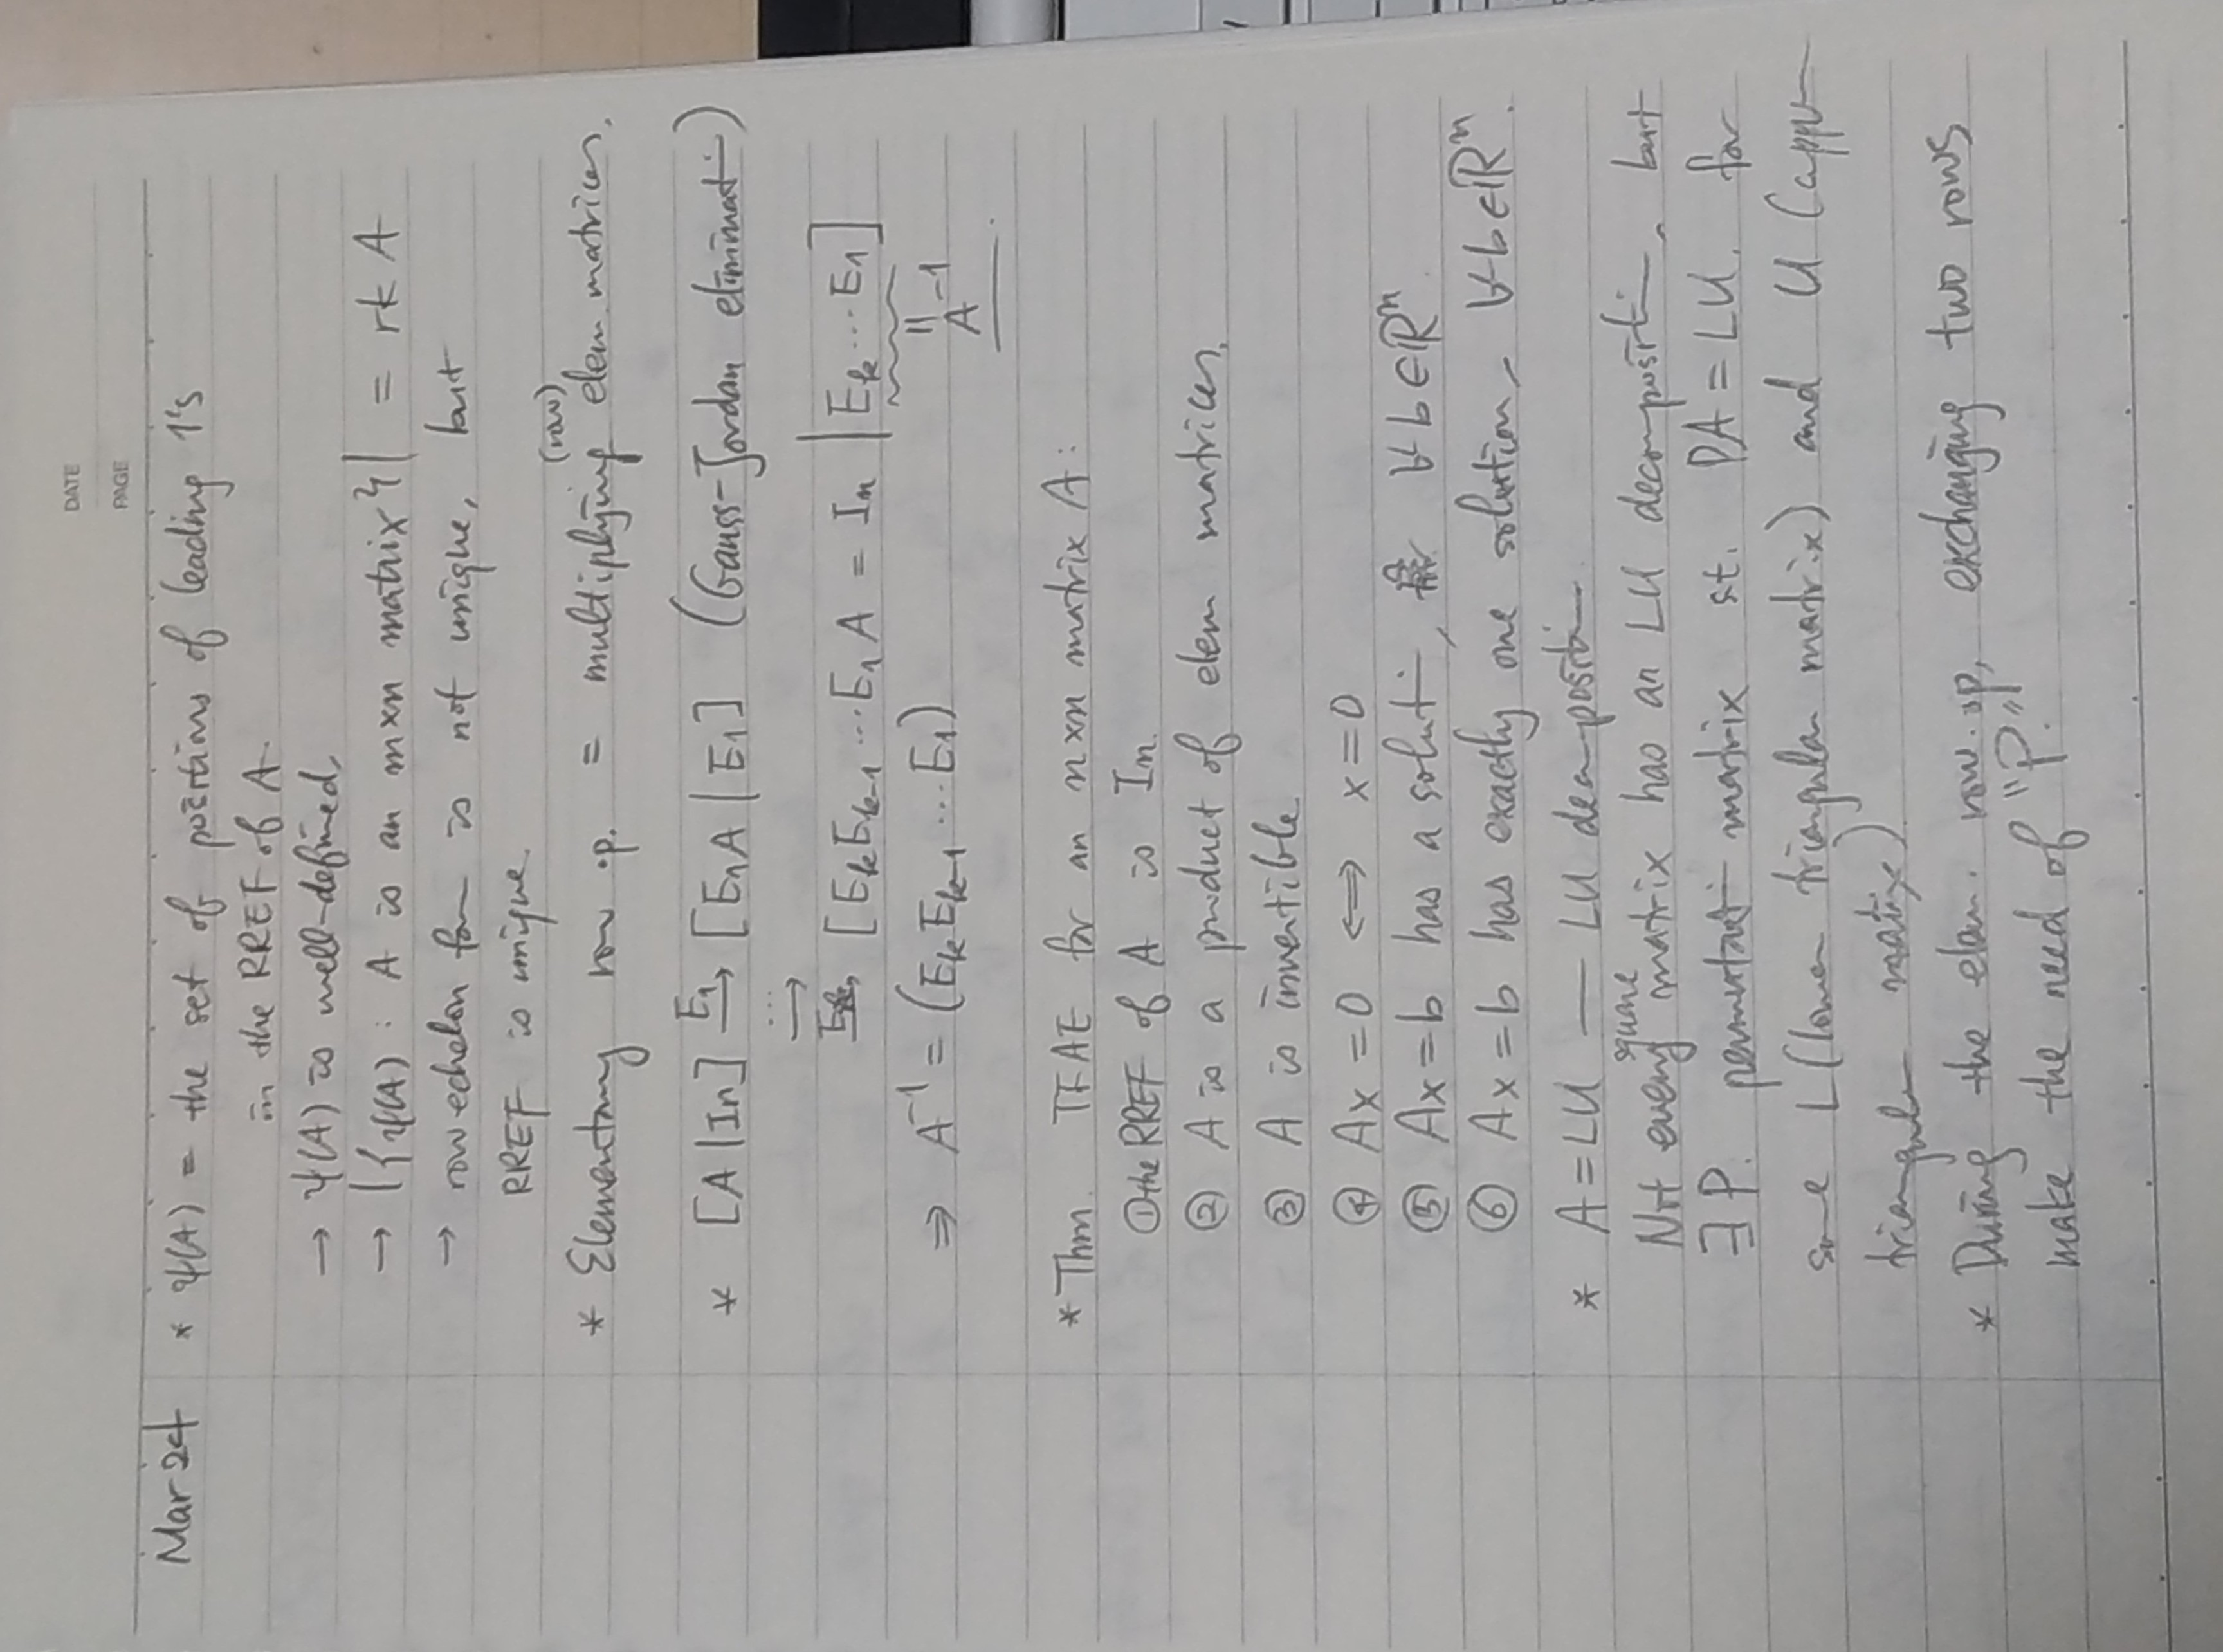
\includegraphics[height=\textwidth,angle=-90,origin=c]{note1.jpg}
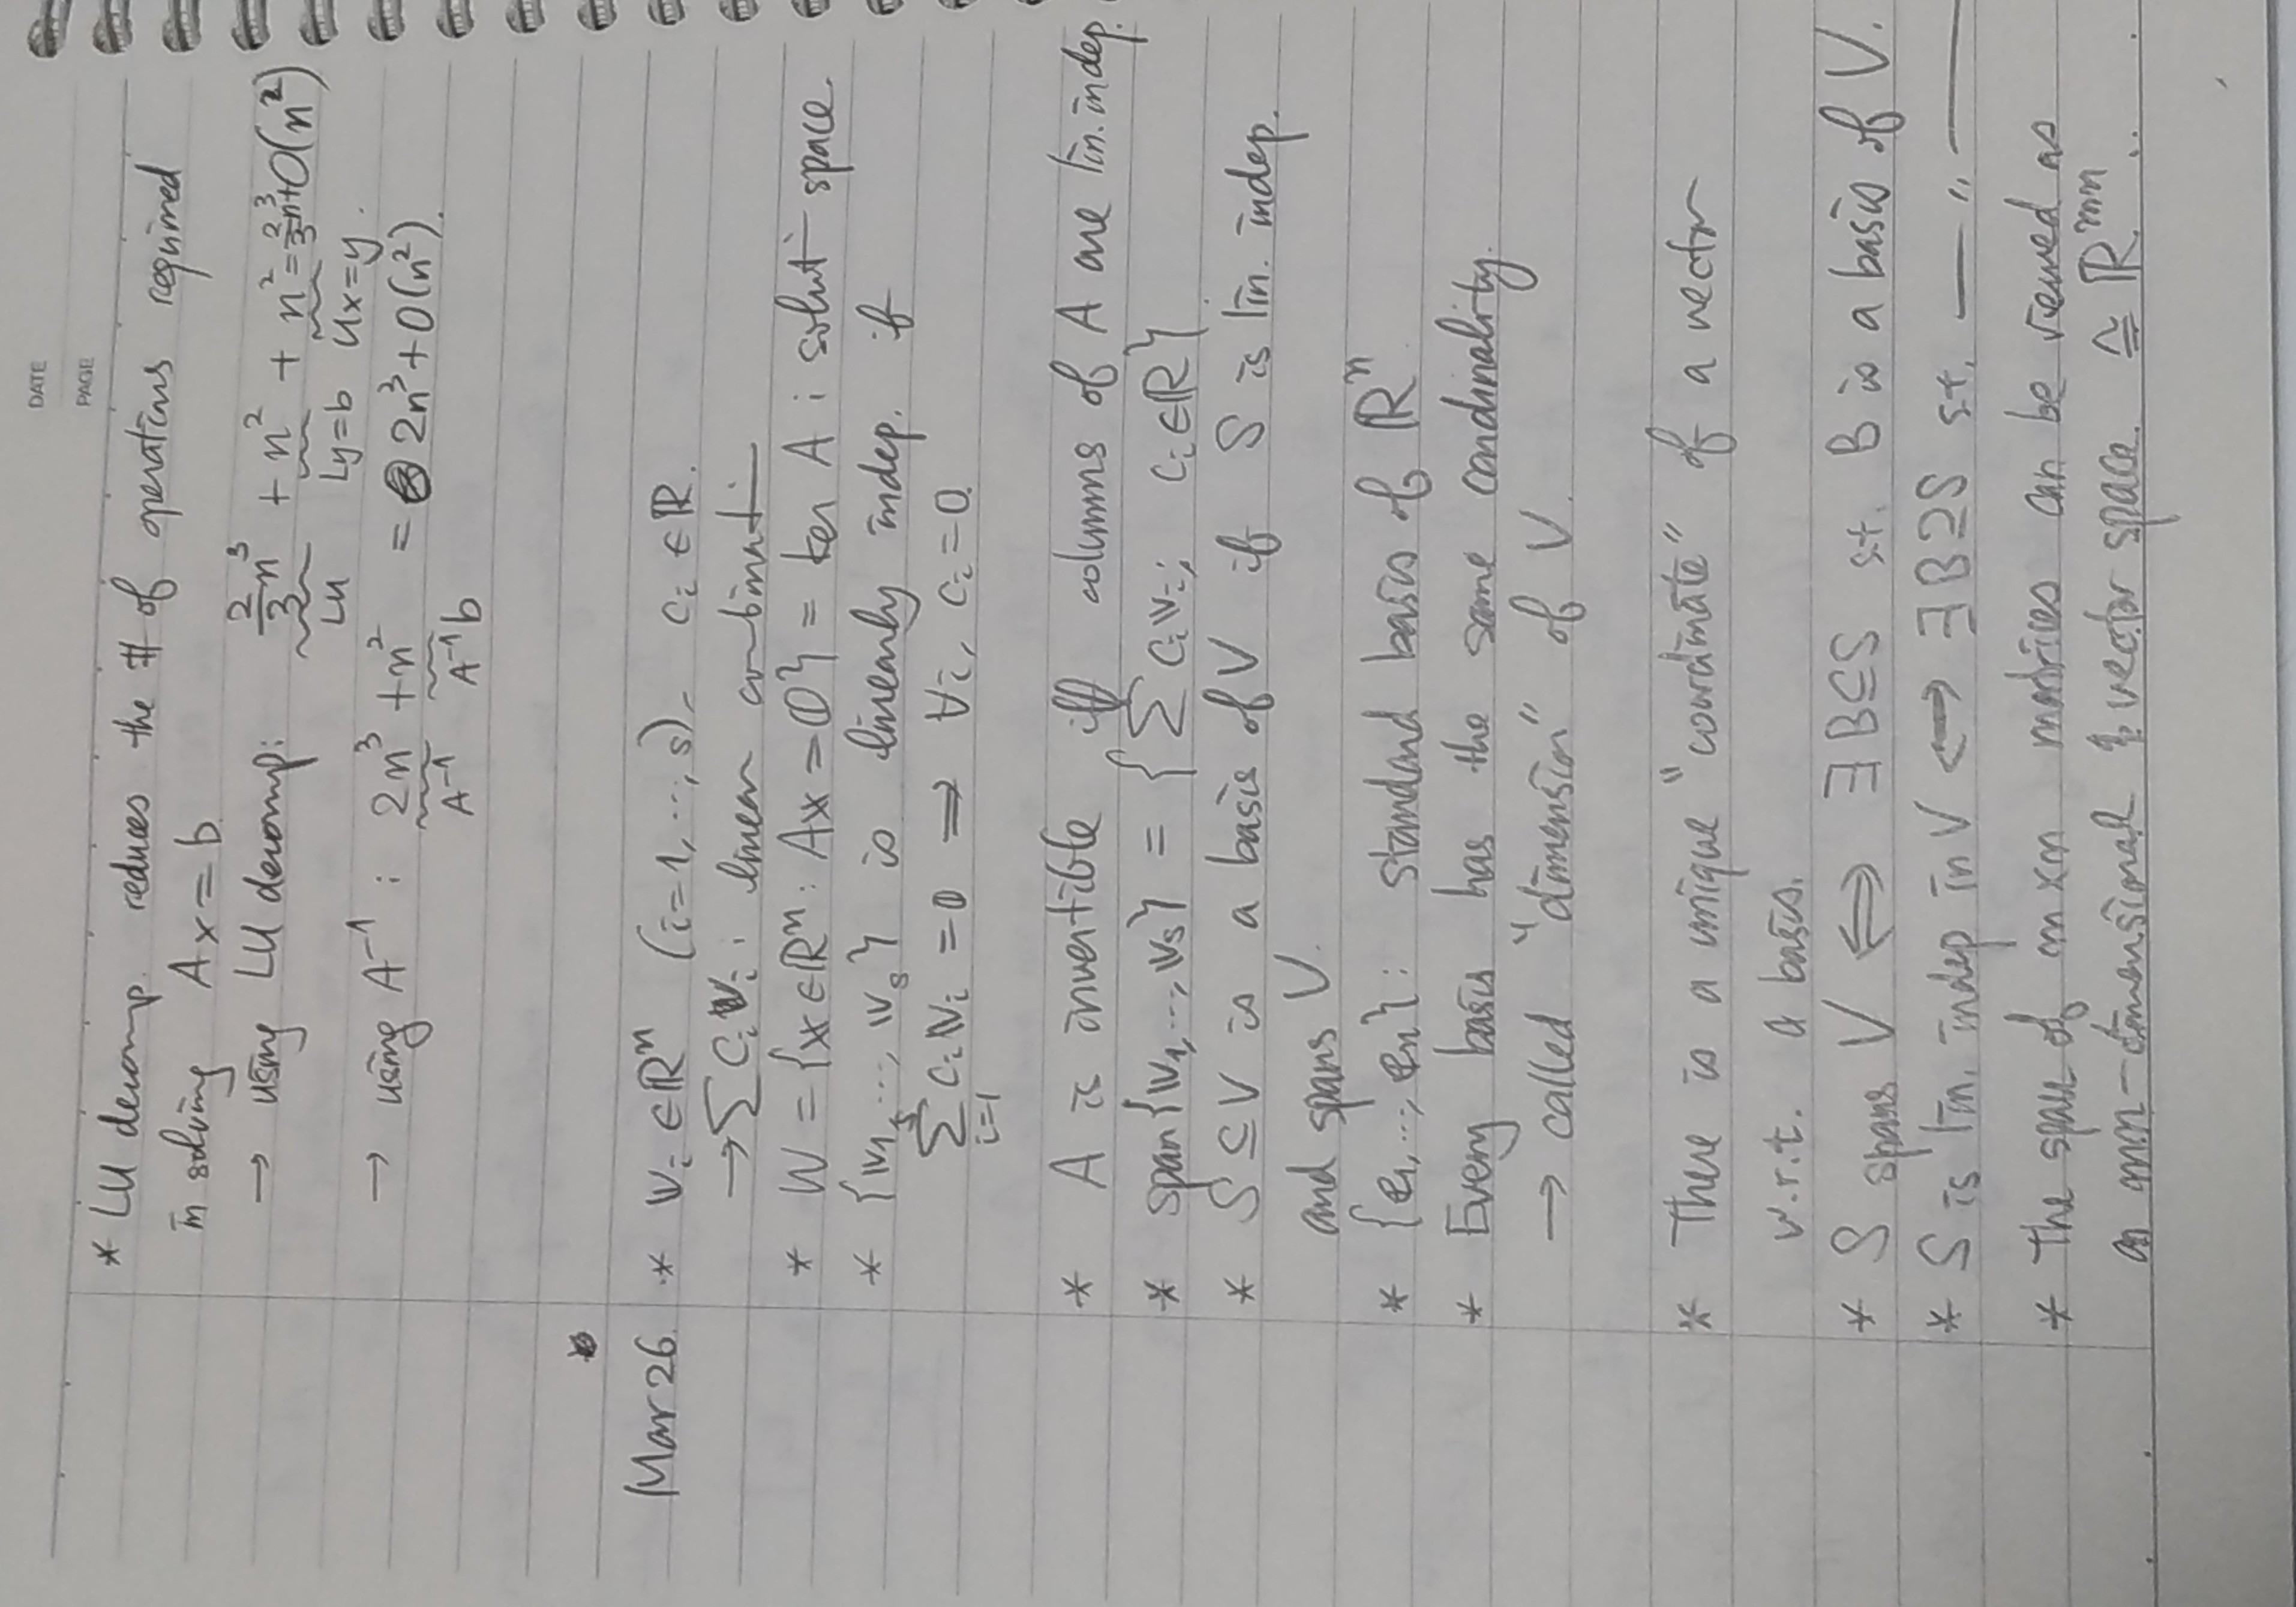
\includegraphics[height=\textwidth,angle=-90,origin=c]{note2.jpg}

\end{document}
